\newpage
\exer{2}

\setcounter{section}{0}

\vspace{0.25cm}


\section{Import}
\begin{prettyBox}{Import}{myblue}
\begin{itemize}
    \item \texttt{numpy} : Les fonctions mathématiques prédéfinies, et \texttt{linspace} pour créer  
        les vecteur des coordonnées x de chaque fonctions.  
    \item \texttt{matplotlib} : Dessine les graphes.  
    \item \texttt{collections} : Crée une nouvelle structure avec \texttt{namedtuple}.  
\end{itemize}
\end{prettyBox}
\vspace{0.5cm}
\lstinputlisting[style=pythonstyle, firstline = 1,lastline=3,basicstyle= \ttfamily\scriptsize]{Exercices/EX2/ex2.py}

\vspace{1cm}

\section{Définition Des Fonctions Mathématiques}
\lstinputlisting[style=pythonstyle, firstline = 8,lastline=12,basicstyle= \ttfamily\scriptsize]{Exercices/EX2/ex2.py}

\vspace{1cm}
\section{\(\epsilon\)}
\lstinputlisting[style=pythonstyle, firstline = 87,lastline=87,basicstyle= \ttfamily\scriptsize]{Exercices/EX2/ex2.py}

\vspace{1cm}
\section{Génération des Vecteurs}
\lstinputlisting[style=pythonstyle, firstline = 89,lastline=94,basicstyle= \ttfamily\scriptsize]{Exercices/EX2/ex2.py}

\newpage
\section{Nouvelle Structure root}
\begin{prettyBox}{root}{myblue}
On a créé une nouvelle structure en utilisant \texttt{namedtuple} root. Elle représente 
les racines pour \( f(x) = 0 \) et possède trois attributs :
\begin{itemize}
    \item \textbf{position} : coordonnée x de la racine
    \item \textbf{a} : extrémité gauche de l'intervalle auquel la racine appartient
    \item \textbf{b} : extrémité droite de l'intervalle auquel la racine appartient
    \item \textbf{error} : Estimation de l'erreur de la method dichotomie.
    \item \textbf{iteration}: Nombre d'iteration de la method dichotomie.
\end{itemize}
\end{prettyBox}
\vspace{0.5cm}
\lstinputlisting[style=pythonstyle, firstline = 5,lastline=5,basicstyle= \ttfamily\scriptsize]{Exercices/EX2/ex2.py}

\vspace{1cm}

\section{Implementation De La Method Dichotomie}
\subsection{Estimation De L'erreur}
\lstinputlisting[style=pythonstyle, firstline = 15,lastline=16,basicstyle= \ttfamily\scriptsize]{Exercices/EX2/ex2.py}

\vspace{0.5cm}
\subsection{Algorithm De Dichotomie}
\lstinputlisting[style=pythonstyle, firstline = 19,lastline=39,basicstyle= \ttfamily\scriptsize]{Exercices/EX2/ex2.py}

\newpage
\section{Dessiner Les Graph \& Racines}
\subsection{Scatter}
\lstinputlisting[style=pythonstyle, firstline = 42,lastline=62,basicstyle= \ttfamily\scriptsize]{Exercices/EX2/ex2.py}

\vspace{0.5cm}

\subsection{Graphes}
\lstinputlisting[style=pythonstyle, firstline = 65,lastline=72,basicstyle= \ttfamily\scriptsize]{Exercices/EX2/ex2.py}

\vspace{1cm}
\section{Tables}
\lstinputlisting[style=pythonstyle, firstline = 75,lastline=85,basicstyle= \ttfamily\scriptsize]{Exercices/EX2/ex2.py}

\newpage
\section{Rest Du Code}
\lstinputlisting[style=pythonstyle, firstline = 96,basicstyle= \ttfamily\scriptsize]{Exercices/EX2/ex2.py}

\vspace{1.5cm}
\section{Figure}
\begin{center}
    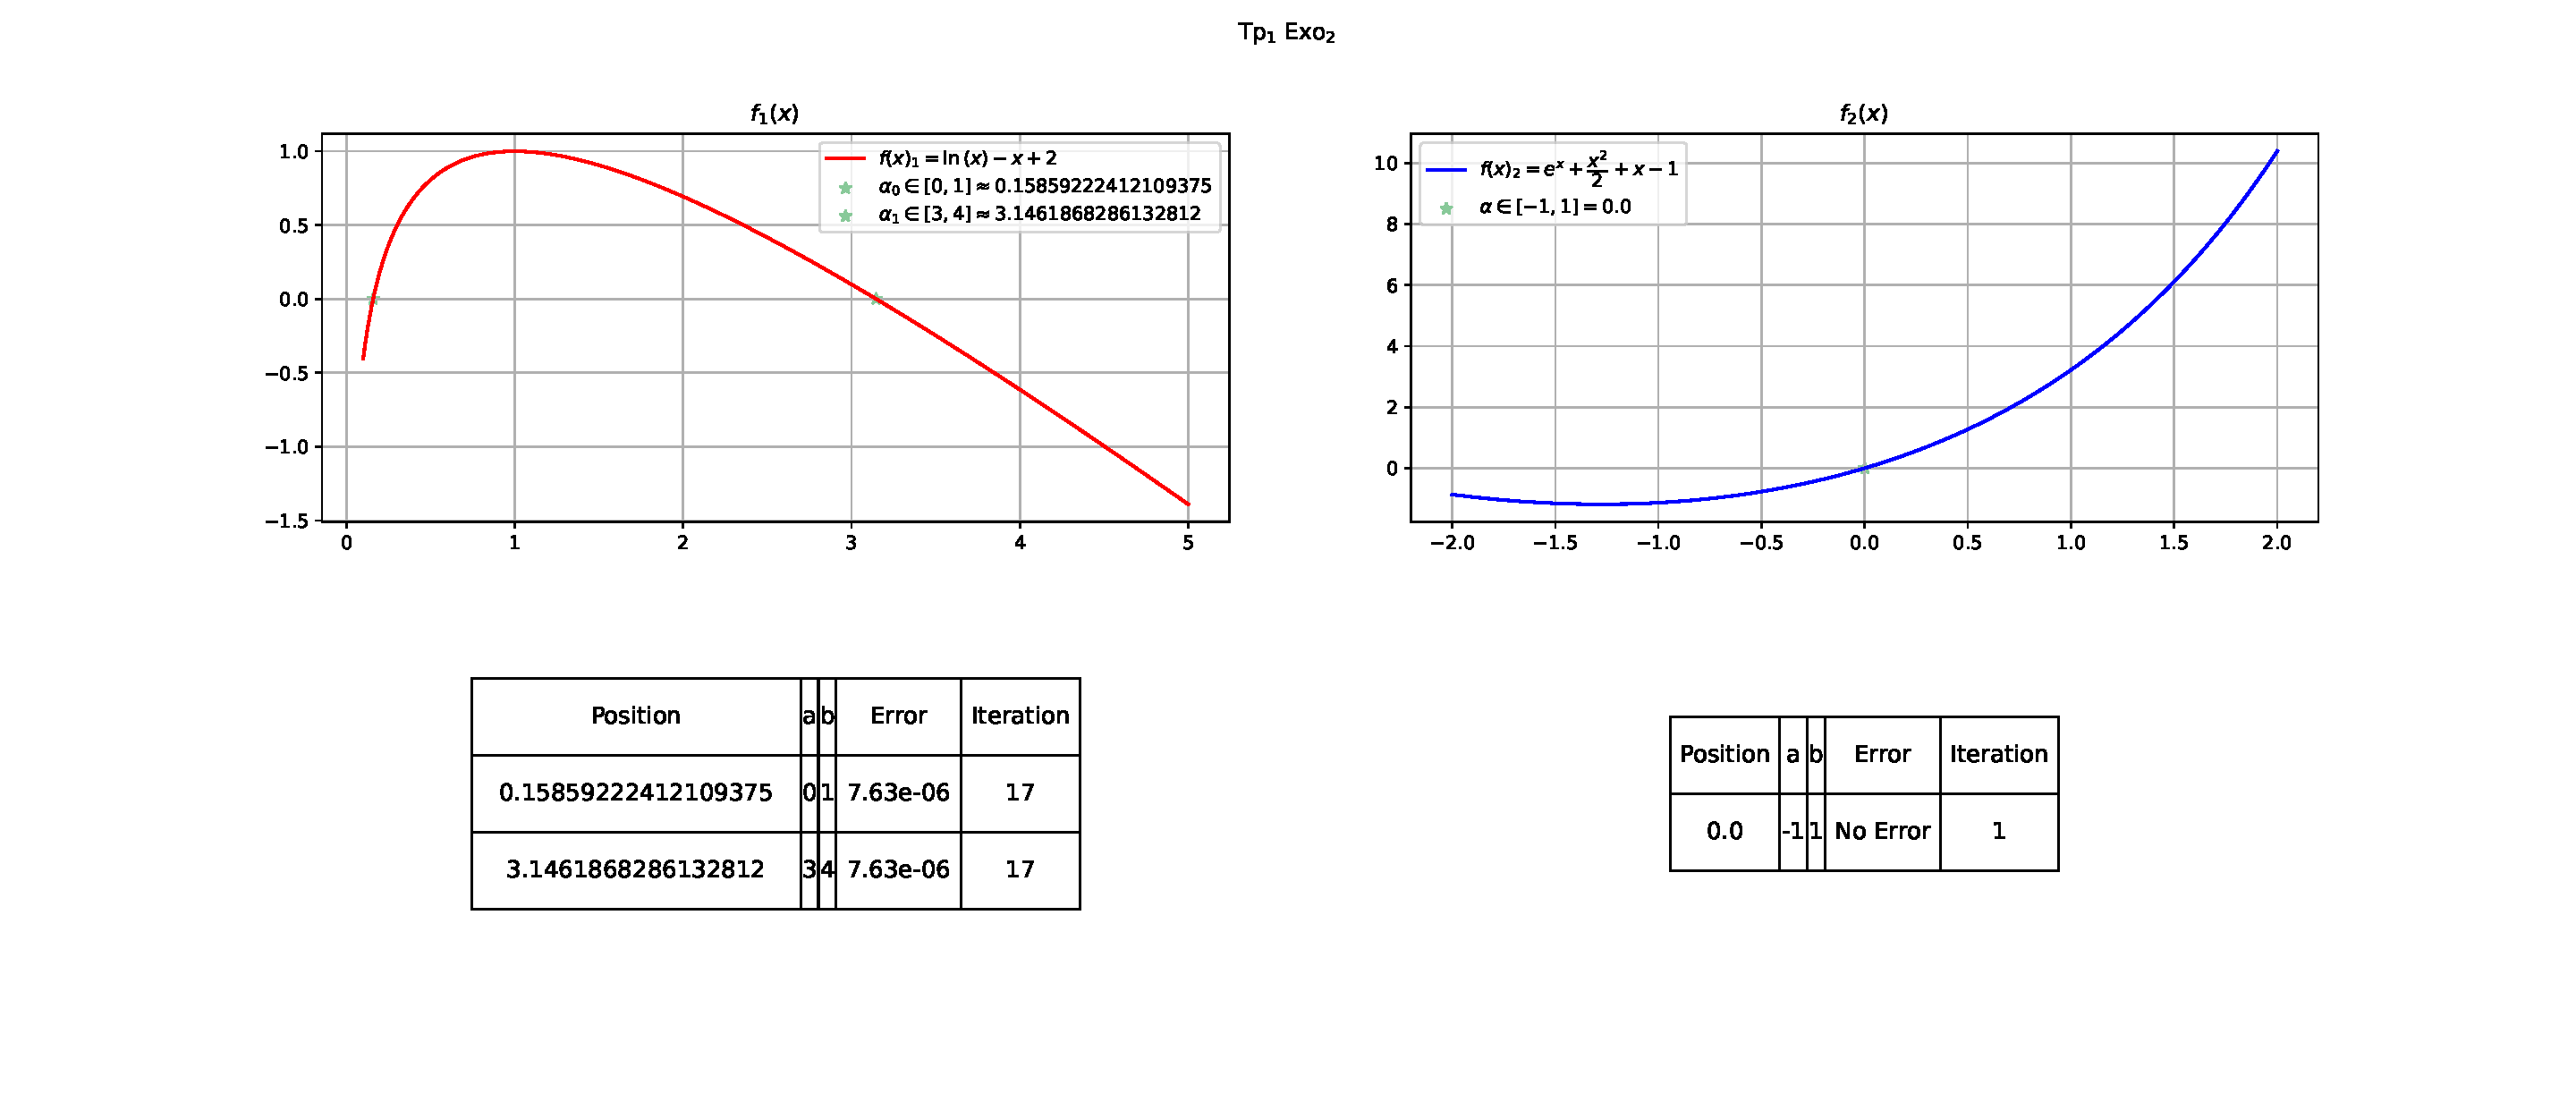
\includegraphics[height=0.35\textheight]{Exercices/EX2/fig.pdf}
\end{center}


